\chapter{Praktischer Teil}
\label{chapter_Praktischer_Teil}
In diesem Kapitel werden die verschiedenen Sensorschaltungen und deren Konfiguration, die Problem
die sich bei der Realisierung ergaben, sowie die Ergebnisse und Auswertungen beschrieben. Außerdem werden die verschiedenen Möglichkeiten zur Datenspeicherung und Visualisierung dargestellt und erklärt. Am Anfang dieses Kapitels werden die zur Realisierung der verschiedenen Aufgaben benötigten Bauteile, kurz etwas näher erklärt und aufgelistet. In Abschnitt \ref{section_DS18S20} wird eine Schaltung mit einem einzigen 1-Wire Temperatursensor aufgebaut, bei der zweiten Schaltung in Abschnitt \ref{section_HTY221} kommt zu dem Sensor aus \ref{section_DB18S20} ein zweiter Temperatursensor und ein Sensor zur Temperaturmessung und Bestimmung der Luftfeuchtigkeit hinzu. Abschnitt (\ref{section_BMA020}) befasst sich mit der Realisierung einer Vibrationsmessung mittels Beschleunigungssensors.

\section{Benötigte Materialien}
\label{section_Benötigte_Materialien}
Die in Tabelle aufgelisteten Materialien wurden für die in Kapitel \ref{chapter_Praktischer_Teil} beschriebenen Versuche verwendet. Bei den einzelnen Sensoren werden die wichtigsten technischen Daten im Anschluss der Tabelle aufgelistet.

%Tabelle 1
\begin{table}[H]
%\rowcolors{2}{black!10}{black!20}
\centering
\begin{tabular}{
lc
}
\toprule
\multicolumn{1}{p{6cm}}{\textit{Bezeichnung}} & \multicolumn{1}{p{3.5cm}}{\centering\textit{Anzahl} } \\\midrule
Raspberry Pi\,3& 1 \\
&\\
Temperatursensor DS18S20 & 2 \\
&\\
Sensor HYT\,221 & 1\\
&\\
3-Achsen-Beschleunigungssensor & 1\\
&\\
Drahtbrücken & mehrere\\
&\\
elektrischer Widerstand 4.7\,$k\Omega$ & 1\\
&\\
Elektronik Steckbrett & 1\\
\bottomrule
\end{tabular}
\caption{benötigte Materialien}
\label{Tabelle_benötigte_Materialien}
\end{table}

\subsection*{DS18S20}
\label{subsection_DS18S20}
Der DS18S20 (siehe Abbildung) ist ein digitaler 1-Wire Temperatursensor, der eine 9\,Bit Temperaturmessung ermöglicht.
Folgend werden die wichtigsten technischen Daten des DB18S20 aufgeführt.

%Abbildund Daten DS18S20
\begin{figure}[!h] 
  \centering
     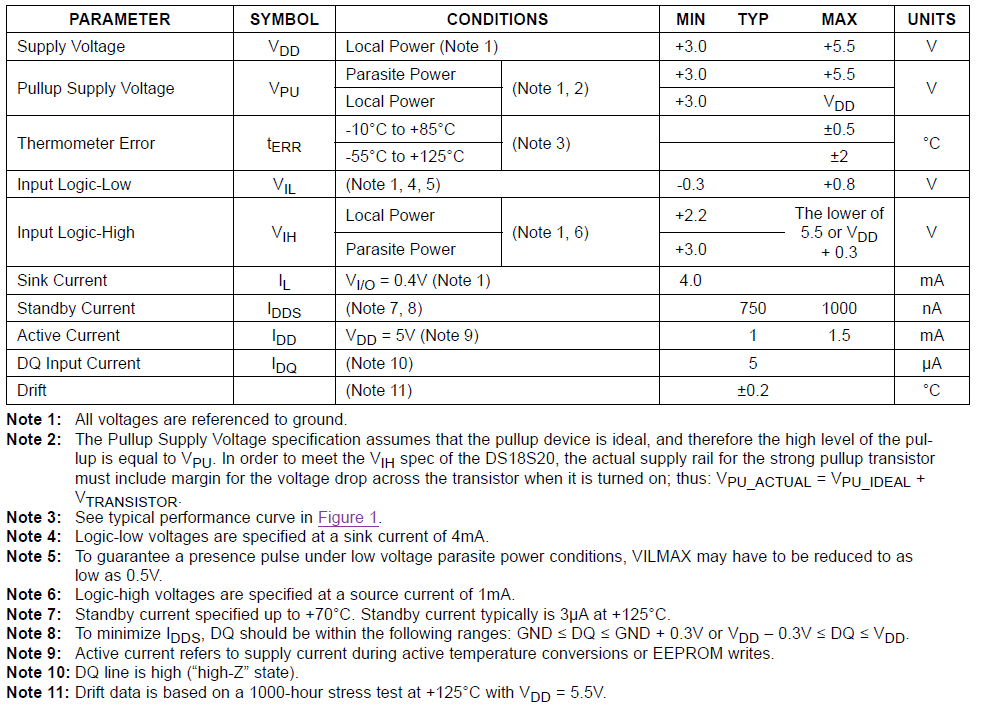
\includegraphics[scale=.6]{BilderAllgemein/Daten_DB18S20.png}
  \caption{elektische Daten DB18S20 \citep[S. 2]{Datenblatt_DB18S20}}
  \label{Abb_elektrische_Daten_DS18S20}
\end{figure}

%Abbildund  DS18S20
\begin{figure}[!h] 
  \centering
     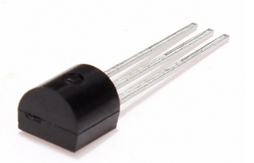
\includegraphics[scale=.8]{BilderAllgemein/DS18S20.png}
  \caption{elektische Daten DB18S20 \citep{Bild_DS18S20}}
  \label{Abb_DS18S20}
\end{figure}

\subsection*{HYT221}
\label{subsection_HYT221}


\section{Temperaturmessung mit Sensor DB18S20}
\label{section_DB18S20}

\section{Temperatur- und Luftfeuchtigkeitsmessung mit HTY221}
\label{section_HTY221}

\section{Vibrationsmessung mit Sensor BMA020}
\label{section_BMA020}